\documentclass[journal,12pt,twocolumn]{IEEEtran}
%

\usepackage{setspace}
\usepackage{gensymb}
\singlespacing

\usepackage{amsmath}
\usepackage{amsthm}
\usepackage{txfonts}
\usepackage{cite}
\usepackage{enumitem}
\usepackage{mathtools}
\usepackage{listings}
    \usepackage{color}                                            %%
    \usepackage{array}                                            %%
    \usepackage{longtable}                                        %%
    \usepackage{calc}                                             %%
    \usepackage{multirow}                                         %%
    \usepackage{hhline}                                           %%
    \usepackage{ifthen}                                           %%
  %optionally (for landscape tables embedded in another document): %%
    \usepackage{lscape}     
\usepackage{multicol}
\usepackage{chngcntr}
\usepackage{tikz}
\usepackage{pgfplots}
\renewcommand\thesection{\arabic{section}}
\renewcommand\thesubsection{\thesection.\arabic{subsection}}
\renewcommand\thesubsubsection{\thesubsection.\arabic{subsubsection}}

\renewcommand\thesectiondis{\arabic{section}}
\renewcommand\thesubsectiondis{\thesectiondis.\arabic{subsection}}
\renewcommand\thesubsubsectiondis{\thesubsectiondis.\arabic{subsubsection}}

% correct bad hyphenation here
\hyphenation{op-tical net-works semi-conduc-tor}
\def\inputGnumericTable{}                                 %%

\lstset{
%language=C,
frame=single, 
breaklines=true,
columns=fullflexible
}

\begin{document}
%


\newtheorem{theorem}{Theorem}[section]
\newtheorem{problem}{Problem}
\newtheorem{proposition}{Proposition}[section]
\newtheorem{lemma}{Lemma}[section]
\newtheorem{corollary}[theorem]{Corollary}
\newtheorem{example}{Example}[section]
\newtheorem{definition}[problem]{Definition}
\newcommand{\BEQA}{\begin{eqnarray}}
\newcommand{\EEQA}{\end{eqnarray}}
\newcommand{\define}{\stackrel{\triangle}{=}}
\bibliographystyle{IEEEtran}
\providecommand{\mbf}{\mathbf}
\providecommand{\pr}[1]{\ensuremath{\Pr\left(#1\right)}}
\providecommand{\qfunc}[1]{\ensuremath{Q\left(#1\right)}}
\providecommand{\sbrak}[1]{\ensuremath{{}\left[#1\right]}}
\providecommand{\lsbrak}[1]{\ensuremath{{}\left[#1\right.}}
\providecommand{\rsbrak}[1]{\ensuremath{{}\left.#1\right]}}
\providecommand{\brak}[1]{\ensuremath{\left(#1\right)}}
\providecommand{\lbrak}[1]{\ensuremath{\left(#1\right.}}
\providecommand{\rbrak}[1]{\ensuremath{\left.#1\right)}}
\providecommand{\cbrak}[1]{\ensuremath{\left\{#1\right\}}}
\providecommand{\lcbrak}[1]{\ensuremath{\left\{#1\right.}}
\providecommand{\rcbrak}[1]{\ensuremath{\left.#1\right\}}}
\theoremstyle{remark}
\newtheorem{rem}{Remark}
\newcommand{\sgn}{\mathop{\mathrm{sgn}}}
\providecommand{\abs}[1]{\left\vert#1\right\vert}
\providecommand{\res}[1]{\Res\displaylimits_{#1}} 
\providecommand{\norm}[1]{\left\lVert#1\right\rVert}
\providecommand{\mtx}[1]{\mathbf{#1}}
\providecommand{\mean}[1]{E\left[ #1 \right]}
\providecommand{\fourier}{\overset{\mathcal{F}}{ \rightleftharpoons}}
\providecommand{\system}{\overset{\mathcal{H}}{ \longleftrightarrow}}
\newcommand{\solution}{\noindent \textbf{Solution: }}
\newcommand{\cosec}{\,\text{cosec}\,}
\providecommand{\dec}[2]{\ensuremath{\overset{#1}{\underset{#2}{\gtrless}}}}
\newcommand{\myvec}[1]{\ensuremath{\begin{pmatrix}#1\end{pmatrix}}}
\newcommand{\cmyvec}[1]{\ensuremath{\begin{pmatrix*}[c]#1\end{pmatrix*}}}
\newcommand{\mydet}[1]{\ensuremath{\begin{vmatrix}#1\end{vmatrix}}}
\newcommand{\proj}[2]{\textbf{proj}_{\vec{#1}}\vec{#2}}
\let\StandardTheFigure\thefigure
\let\vec\mathbf
\title{Assignment - 1}
\author{V Krishna Kanth Makena
\\ MD/2020/711}
% make the title area
\maketitle
\newpage
%\tableofcontents
\bigskip
\renewcommand{\thefigure}{\theenumi}
\renewcommand{\thetable}{\theenumi}
%\renewcommand{\theequation}{\theenumi}
\begin{abstract}
This is a simple document to learn about writing vectors and matrices using latex, draw figures using Python, Latex.
\end{abstract}
%Download all python codes 
%
%\begin{lstlisting}
%svn co https://github.com/JayatiD93/trunk/My_solution_design/codes
%\end{lstlisting}
Download all and latex-tikz codes from 
%
\begin{lstlisting}
svn co https://github.com/MVKKanth/Assignment-1
\end{lstlisting}
%
question taken from
\section{Vectors}
%
\begin{lstlisting}
(cbse/math/10/2008/qp-math-x-2008.pdf Code 30/2/1 - Q21)}\end{lstlisting}
%
\renewcommand{\theequation}{\theenumi}
\begin{enumerate}[label=\thesection.\arabic*.,ref=\thesection.\theenumi]
\numberwithin{equation}{enumi}
\item If $\vec{P}$ divides the join of $\vec{A}\myvec{-2\\-2}$ and $\vec{B}\myvec{2\\-4}$ such that $\frac{\vec{AP}}{\vec{AB}} = \frac{3}{7}$, \textrm find the coordinates of $\vec{P}$.
\\
\solution\begin{enumerate}
    \item Let 
    \begin{align}
     \vec{P}=\myvec{x\\y}   
    \end{align}
    We have \begin{align}
    \vec{A}=\myvec{-2\\-2},
    \vec{B}=\myvec{2\\-4}
    \end{align}
    and
    \begin{align}
        \frac{AP}{AB} &= \frac{3}{7}\\
        \implies \frac{AP}{PB} &= \frac{3}{4}\\
        \end{align}
        
         So, the coordinates of the point 
         \begin{align}
             \vec{P}\myvec{x\\y} 
         \end{align}
         which divides the line segment joining the points 
         \begin{align}
             \vec{A}\myvec{x1&y1}\\ \vec{B} \myvec{x2&y2}
         \end{align}
         internally, in the ratio m1 : m2 are 
         \begin{align}
             \frac{(m1x2 + m2x1)}{(m1 + m2 )},\frac{(m1y2 + m2y1)}{(m1 + m2 )}
         \end{align}
         This is known as the section formula.\\ \\
          Given\\
        \begin{align}
            \vec{m1}: \vec {m2} = 3:4\\
            \vec{p}\myvec{x&y}= \myvec{\frac{3(2)+4(-2)}{4+3},\frac{3(-4)+4(-2)}{4+3}}\\
            \implies\myvec{\frac{-2}{7} \frac{-20}{7}}
        \end{align}

\begin{figure}[h]
\centering
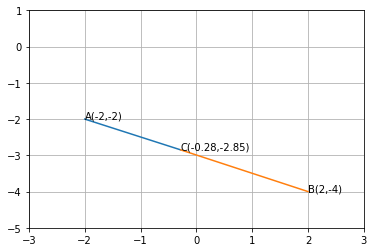
\includegraphics[width=\columnwidth]{1.1.png}
\label{Fig 1.1.png}
\caption{Two lines representing given equations meet at point $\myvec{\frac{-2}{7}&\frac{-20}{7}}$}.
\end{figure}
\end{enumerate}
\end{document}